\paragraph{Software tools}
We use the FastICA algorithm~\cite{hyvarinen_fast_1999} to perform independent component analysis and use $k=900$ components. We use Nilearn~\cite{abraham_machine_2014} for fMRI
processing, Scikit-learn~\cite{pedregosa2011scikit},
Numpy~\cite{harris2020array} and Scipy~\cite{2020SciPy-NMeth} for data
manipulation and machine learning tools.

\paragraph{Code availability}
Our code is available on the following git repository:
\url{https://github.com/hugorichard/fmriaugment}.
%


\section{Experiments}
\subsection{Dataset, data augmentation baselines and classifiers used}
The unmixing matrices are learned on the rest HCP
dataset~\cite{van2013wu} using 200 subjects.
These data were used after standard
preprocessing, including linear detrending, band-pass filtering
($[0.01, 0.1]Hz$) and standardization of the time courses.
The other 8 datasets~\cite{van2013wu, shafto2014cambridge,
  orfanos2017brainomics, pinel2019functional, pinel2007fast, pinel2013genetic,
  poldrack2016phenome, pinel2013genetic} are obtained from the Neurovault repository~\cite{gorgolewski2015neurovault}.
The classes used in each dataset correspond to the activation maps
related to the contrasts (such as ``face vs tools'')
present in the set of tasks of each dataset. Details are available in
appendix Table~\ref{app:dataset:tab}.

We consider 5 alternative
augmentation methods: \emph{ICA}, \emph{Covariance}, \emph{ICA + Covariance}, \emph{GANs} and \emph{CGANs}.
%
When no augmentation method is applied we use the label \emph{Original}.

The \emph{ICA} covariance method applies ICA to $X^{task}$ to generate unmixing matrices $W^{task}$ and
components $S^{task}=  W^{task} X^{task}$.
%
To generate a sample $\tilde{\xb}_c$ from class $c$, we sample
independently from each component restricted to the samples of class $c$ yielding $\tilde{\sbb}^{task}_c$ and mix the data: $\tilde{\xb}_c = (W^{task})^{\dagger}
\tilde{\sbb}^{task}_c$.
%

The \emph{Covariance} method generates a new sample of
synthetic data in class $c$ by sampling from a Multivariate Gaussian
with mean $\mub_c$ and covariance $Sigma$, where $\mub_c$ is the
class mean and $Sigma$ is the covariance of centered task data
estimated using Ledoit-Wolf method.
%
In brief, it assumes normality of the data per class.

The \emph{ICA + Covariance} method combines the augmentation
methods \emph{ICA} and \emph{Covariance}: samples are drawn following
the ICA approach, but with some additive non-isotropic Gaussian noise.
%
As in \emph{ICA} we estimate $W^{task}$ and $S^{task}$ from
$X^{task}$ via ICA.
%
Then we consider $R_{task} = X_{task} - W_{task} S_{task}$ and estimate the
covariance $Sigma_R$ of $R_{task}$ via LedoitWolf's method.
%
We then generate a data sample $\tilde{\xb}_c$ from class $c$ as with ICA and add
Gaussian noise $\tilde{\nb} \sim \mathcal{N}(0,Sigma_R)$.
%
Samples are thus generated as $\tilde{\xb}_c + \tilde{\nb}$.

The \emph{GANs} (respectively \emph{CGANs}) method use a GANs (respectively CGANs) to generate data. The generator and discriminator have a mirrored architecture with 2 fully connected hidden layer of size (256 and 512).  The number of epochs, batch size, momentum and learning rate are set to 20k, 16, 0.9, 0.01 and we use the Leaky RELU activation function.

We evaluate the performance of augmentation methods through the use of classifiers: logistic regression (LogReg), linear
discriminant analysis with Ledoit-Wold estimate of covariance (LDA) perceptron
with two hidden layers (MLP) and random forrests (RF).
The hyper-parameters in each classifier are optimized through an internal 5-Fold
cross validation. We set the number of iterations in each classifier so that
convergence is reached. The exact specifications are available in appendix Table~\ref{app:classifiers:tab}.


 
\subsection{Distinguish fake from real HCP resting state data}
This experiment is meant to assess the effectiveness of the data
augmentation scheme in producing good samples.
Data augmentation methods are trained on 200 subjects taken from HCP rest fMRI
dataset which amounts to $960k$ samples (4800
per individual). Then synthetic
data corresponding to $200$ synthetic subjects are produced, yielding
$960k$ fake samples and various classifiers are trained to distinguish fake from
real data using 5-Fold cross validation. The cross-validated accuracy is shown
in Table~\ref{tab2}.
Interestingly, we observe a dissociation between linear models (LogReg
and LDA) that fail to discriminate between generated and actual data,
and non-linear models (MLP and RF) that can discriminate samples from
the alternative augmentation methods.
%
By contrast, all classifiers are at chance when Conditional ICA is used.

\begin{table}
\begin{center}
\begin{tabular}{c|cccc}
\hline
Models & LDA  & LogReg & Random Forest &  MLP 
\\ \hline
ICA   & 0.493 & 0.500 & 0.672 &  0.697
\\
Covariance   & 0.473 & 0.461 & 0.610 &  0.626
\\
ICA + Covariance   & 0.509 & 0.495 & 0.685 &  0.706
\\
GANs   & 0.501 & 0.498 & 0.592 &  0.607
\\
CGANs   & 0.498 &  0.493 & 0.579 & 0.604
\\\hline
\textbf{Conditional ICA}  & 0.503 & 0.489 & 0.512 &  0.523
\\\hline\hline
\end{tabular}
\end{center}
  \caption{\textbf{Distinguish fake from real HCP resting state data}
    We use HCP resting state data from $n=200$ subjects ($960k$ samples) and produce an equally
    large amount of fake data ($960k$ samples) using data augmentation methods.
    The table shows the 5-fold cross validated accuracy obtained with various
    classifiers. When Conditional ICA is used, all classifiers are at chance.
    %
    }\label{tab2}
\end{table}
%
\subsection{Comparing augmentation methods based on classification accuracy on task
  HCP dataset}
In order to compare the different augmentation methods, we measure their 
relative benefit in the context of multi-class classification.
We use 787 subjects from the HCP task dataset that contains 23 classes and
randomly split the dataset into a train set that contains 100 subjects and a test set
that contains 687 subjects. In each split we train augmentation methods on the
train set to generate fake samples corresponding to $200$ subjects.  
These samples are then appended to the train set, resulting in an
augmented train set on which the classifiers are trained. Results, displayed in Table~\ref{tab3}, show that Conditional ICA always yields a higher accuracy  than when no augmentation method is applied. The gains are over 1\% on all classifiers tested. 
%
By contrast, ICA+Covariance and ICA lead to a decrease in accuracy
while the Covariance approach leads to non-significant
gains.
%
To further investigate the significance of differences between the proposed approach and other state-of-the-art methods, we perform a t-test for paired samples (see Table~\ref{app:significance} in appendix). Most notably, the proposed method performs significantly better than other data augmentation techniques. Given the large size of the HCP task data evaluation set, this significance test would demonstrate that the gains are robust.
%
Note that the random forest classifier is not used in this experiment as it leads to a much lower accuracy than other methods. For completeness, we display the results obtained with random forest in appendix Table~\ref{app:randomforrest}.

Visualization of fake examples produced by GANs, CGANs and Conditional ICA are available in appendix Figure~\ref{app:visualization:fig}.
%
\begin{table}[!b]
  \setlength{\tabcolsep}{0.23em}
%{\renewcommand{\arraystretch}{1}% for the vertical padding
\begin{center}
  \begin{tabular}{c|c|c|c}
    \hline
    Models & LDA & LogReg & MLP \\
    \hline
    Original           & 0.893 & 0.874 &  0.779 \\
    ICA                & 0.814 & 0.840 &  0.803 \\
    Covariance         & 0.895 & 0.876 &  0.819 \\
    ICA + Covariance   & 0.816 & 0.840 &  0.815 \\
    GANs               & 0.877 & 0.863 &  0.771 \\
    CGANs              & 0.874 & 0.874 &   0.726 \\
    \hline
    \textbf{Conditional ICA} &  \textbf{0.901} & \textbf{0.890} & \textbf{0.832} \\
    \hline\hline
\end{tabular}
\end{center}
\caption{\textbf{Comparing augmentation methods based on classification accuracy on task
      HCP dataset} We compare augmentation methods based on the classification
    accuracy \textbf{(Acc)} obtained by 2 linear classifiers (LDA and LogReg) and one
    non-linear classifier trained on augmented datasets on HCP
  Task fMRI data. We report the mean accuracy across 5 splits.}\label{tab3}
\end{table}




\subsection{Gains in accuracy brought by conditional ICA on eight datasets.}

In this experiment we assess the gains brought by Conditional ICA data
augmentation on eight different task fMRI dataset. The number of subjects,
classes and the size of train and test set vary between dataset and are reported
in appendix Table~\ref{app:classifiers:tab}. The rest of the experimental pipeline is exactly the same as with the HCP task dataset.
We report in Fig.~\ref{Fig4} the cross-validated accuracy of
classifiers with and without augmentation.
We notice that the effect of data augmentation is
consistent across datasets, classifiers and splits, with 1\% to 5\% net gains.
%
\begin{figure}
  \centering
  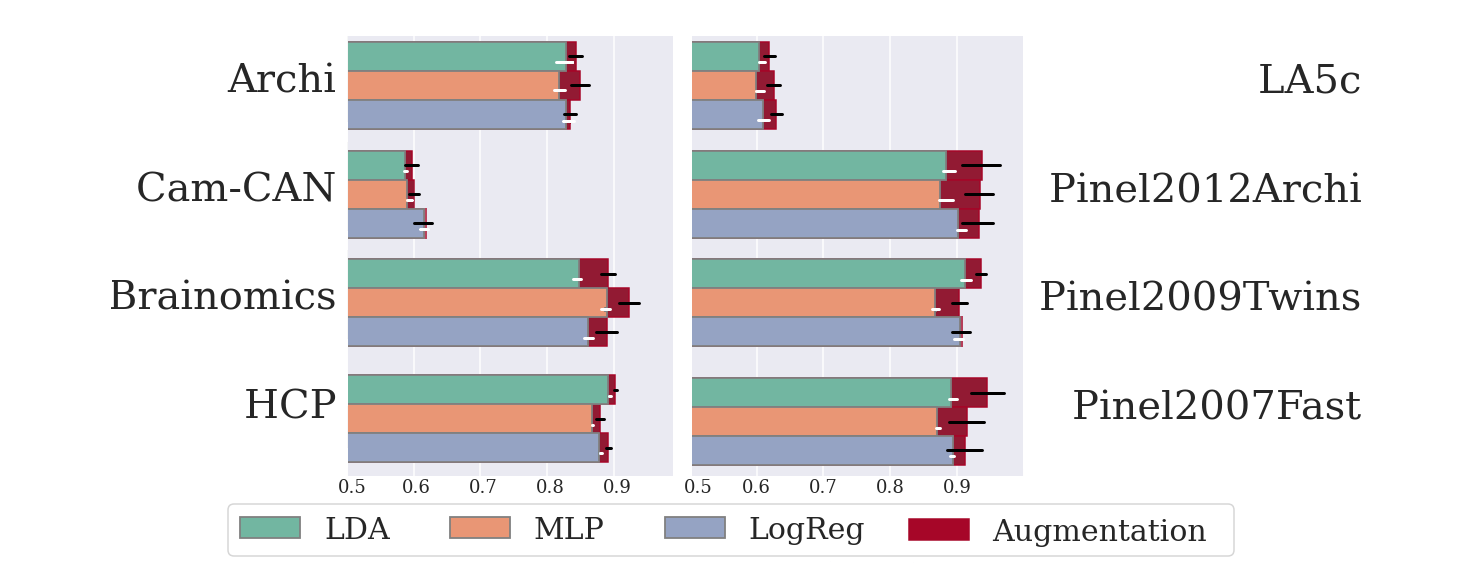
\includegraphics[width=\textwidth]{figures/condica/accuracy_all_datasets_v5.png}
\caption{\textbf{Accuracy of models for eight multi-contrast datasets.} Cross
  validated accuracy of two linear (LDA and LogReg) and one non-linear
  classifier (MLP) with or without using data augmentation.
  %
  The improvement yielded by data augmentation is displayed in red.
  %
  Black error bars indicate standard deviation across splits while white error bars indicate standard deviation across splits with no augmentation.}
\label{Fig4}
\end{figure}
%
An additional experiment studying the sensitivity of Conditional ICA to the
number of components used is described in appendix Figure~\ref{app:sensitivity:fig}.

\section{Discussion \& Future work}
In this work we introduced Conditional ICA a fast generative model
for rest and task fMRI data. It produces samples that cannot be distinguished from true actual rest by 
linear as well as non-linear classifiers, showing that it captures higher-order statistics than naive ICA-based generators.
%
When Conditional ICA is used as a data augmentation method, it yields consistent
improvement in classification accuracy: on 8 tasks fMRI datasets, we observe
increase in accuracy between 1\% and 5\% depending on the dataset and the
classifier used.
Importantly, this performance was obtained without any fine-tuning of
the method, showing its reliability. One can also notice that our experiments cover datasets with different cardinalities, from tens to thousand, and different baseline prediction accuracy.
It is noteworthy that Conditional ICA is essentially a linear
generative model with pointwise non-linearity, which makes it cheap,
easy to instantiate on new data, and to introspect.

%
The speed and simplicity of Conditional ICA
as well as the systematic performance improvement it yields
make it a promising candidate for data augmentation in a wide range of
contexts. Future work may focus on its applicability to other decoding tasks
such as the diagnosis of Autism Spectrum Disorder
(ASD)~\cite{eslami2019asd,eslami2019auto,dvornek2017identifying} or
Attention-Deficit/Hyperactivity Disorder detection (ADHD)~\cite{mao2019spatio}. Other extensions of the present work concern the adaptation to
individual feature (e.g. age) prediction where
fMRI has shown some potential.
%